\section{Einfluss im Leerlauf befindlicher Schienen auf die Ringkernimpedanz}
Es sollte nicht au\ss{}er Acht gelassen werden, dass vorab montierte Kurzschlussschienen in der Testbox oder der Kavit\"at im laufenden Betrieb nicht einfach wieder entfernt werden k\"onnen. Es stellt sich die Frage, ob diese auch eine Auswirkung auf die Ringkernimpedanz haben, wenn sie nicht kurzgeschlossen sind. Im folgenden Abschnitt soll daher analysiert werden, ob auch Schienen, welche sich im Leerlauf befinden, einen Einfluss auf die Impedanz haben. Abbildung~\ref{fig:openksnumber} zeigt das Verhalten der eingebrachten Schienen im Leerlauf.
\begin{figure}[htb]
	\centering
	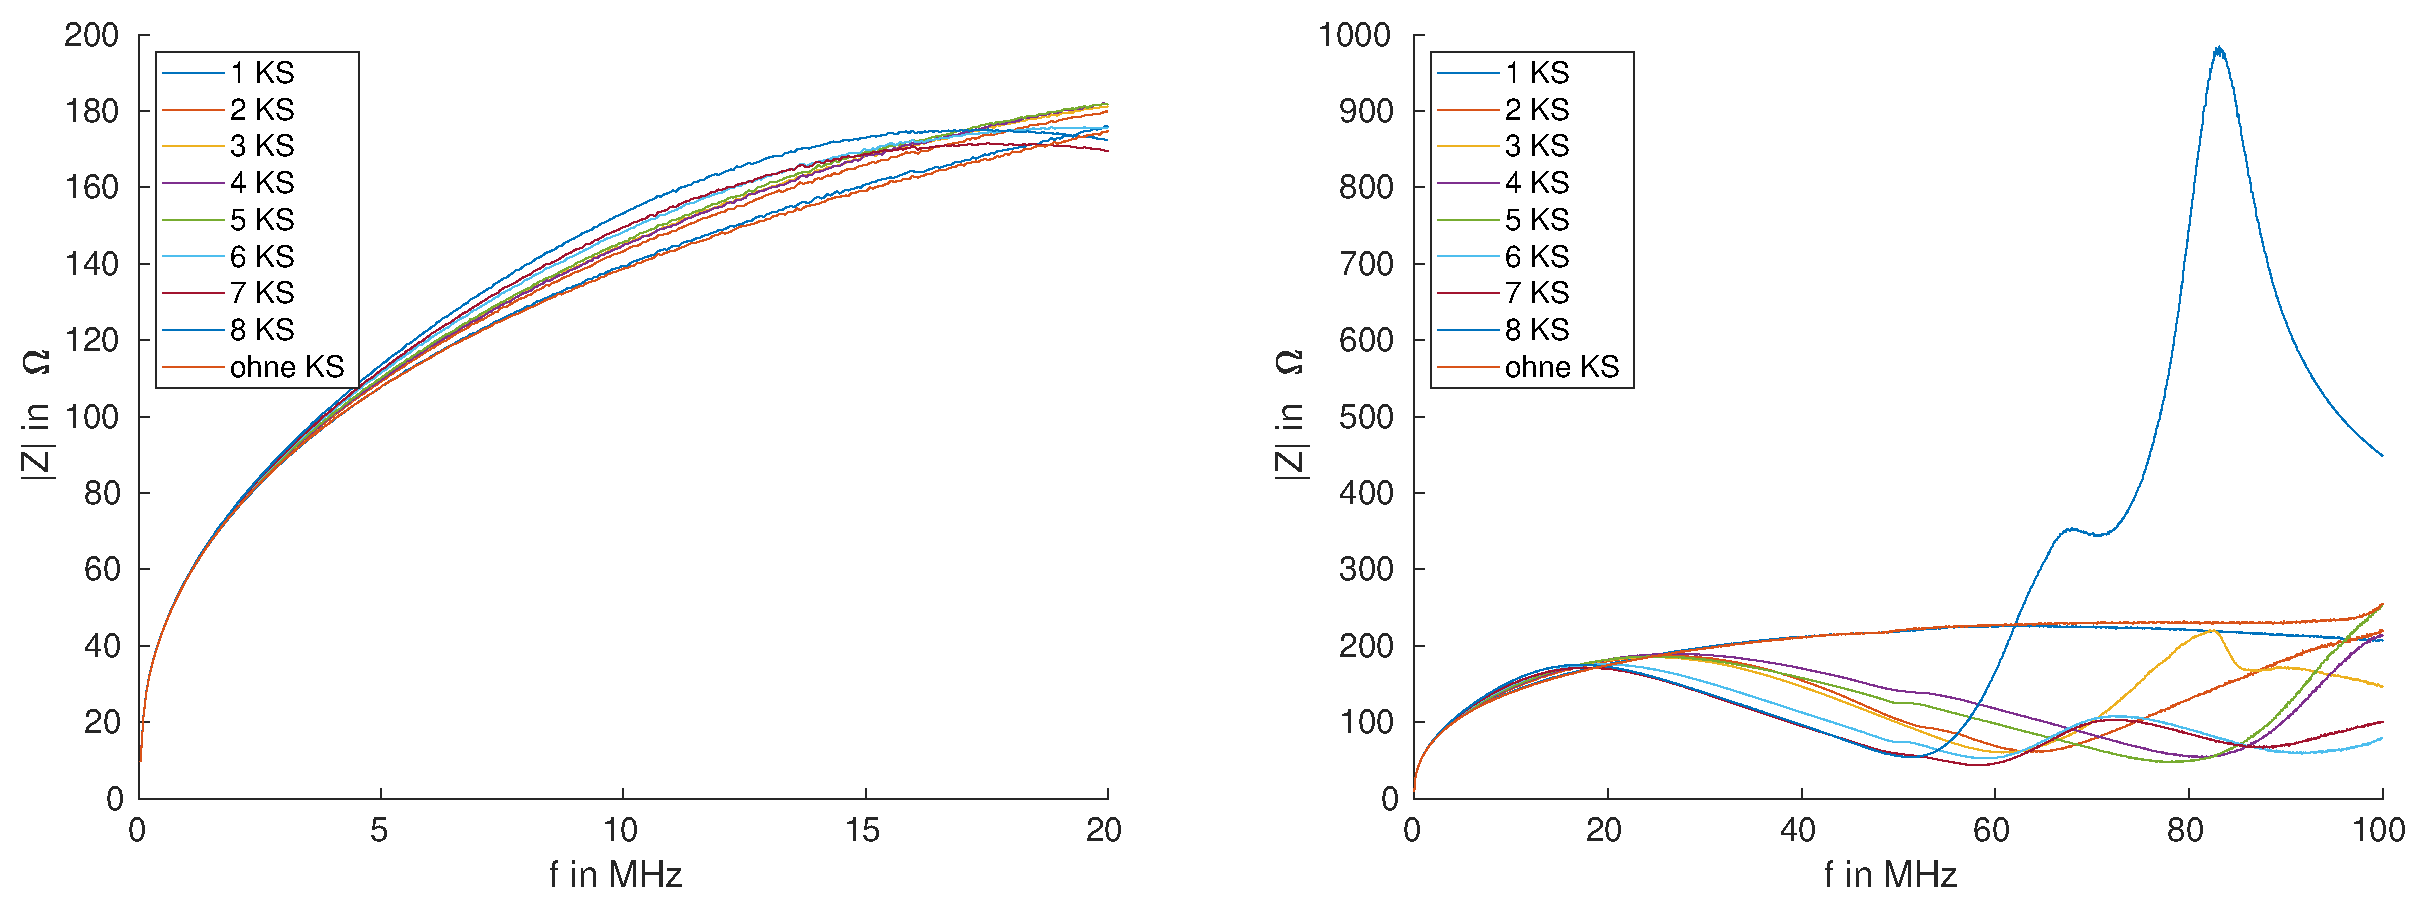
\includegraphics[width=\textwidth]{Z_RK_numKS_open}
	\caption{Gegen\"uberstellung der Ringkernimpedanz \"uber der Frequenz f\"ur verschiedene Anzahlen an offenen Kupferschienen.}
	\label{fig:openksnumber}
\end{figure}
\par
Es wird deutlich, dass die Schienen im Frequenzbereich unter $\SI{20}{\mega\hertz}$ kaum einen Einfluss haben. Der Extremfall bei $\SI{20}{\mega\hertz}$ liefert nach Gleichung~\ref{eq:maxdiffpercent} eine \"Anderung von rund $\SI{2,6}{\%}$ der Ringkernimpedanz f\"ur eine Anordnung mit zwei Kurzschl\"ussen gegen\"uber einer Anordnung ohne Kurzschl\"usse. Somit ist davon auszugehen, dass die Kurzschl\"usse den Betrieb nicht st\"oren, sofern diese gut genug getrennt werden.